\documentclass[a4paper]{report}
\author{Jure Kos}
\title{Vaja 47, Sila med ploščama kondenzatorja}
\date{3.3.2022}
\usepackage{graphicx}
\graphicspath{ {./images/} }

\begin{document}


\maketitle

\chapter*{Uvod}

Privlaka med elektrodama kondenzatorja je posledica električnih privlačnih sil med nasprotnima nabojema. To si ogledamo pri ploščatem kondenzatorju, ki ima plošči s ploščino S v razmiku d. Kapaciteta kondenzatorja je tedaj $C=\epsilon_0S/d$. Na ploščo pritisnemo napetost U. Sila (F) med ploščama kondenzatorja je enaka produktu naboja na prvi plošči ter poljske jakosti, ki bi jo dobili samo z nabojem na drugi plošči. To izrazimo po formuli:
$F=e_1 E_2$
Upoštevati je potrebno $e_1=CU$, vrednost $E_2= \frac{U}{2d}$.
Z izrazom za kapaciteto lahko izračunamo silo F:
$F= \frac{CU^2}{2d}= \frac{\epsilon_0 SU^2}{2d^2}$
Tudi pri drugače oblikovanih elektrodah je kvadrat napetosti sorazmeren s silo. Silo med elektrodama pa v statičnih voltmetrih lahko izkoriščamo za merjenje napetosti. 

\chapter*{Naloga}
Izmeri silo med ploščama danega kondenzatorja v odvisnosti od napetosti in določi električno konstanto. \\
Nariši diagram $F = F(U^2)$. Iz strmine premice, ki se najbolje prilega meritvam, izračunaj $\epsilon_0$. Primerjaj rezultat z vrednostjo $\epsilon_0 = (c^2\mu_1)^{-1}$ , kjer je $\mu_0 = 4\omega \cdot 10^{-7} Vs/A in c = 2,998\cdot 108 m/s$ (svetlobna hitrost).

\section*{Potrebščine}
1. Tehtnica s kondenzatorskima ploščama,\\
2. usmernik za 2000 V, \\
3. voltmeter, \\
4. 2 žici.

\chapter*{Meritve}

polmer plošče = $9.5cm \pm 0.2cm $\\
razmik med ploščama = $0.51cm \pm 0.01cm$ \\
\\


    \begin{center}
    \begin{tabular}{|c|c||c|c|}
    \hline
    U(V) & m(mg)&       U(V) & m(mg) \\
    \hline
    4,60 & 500  &       9,16 & 1200 \\
    4,54 & 500  &       9,01 & 1200 \\
    4,70 & 500  &       8,80 & 1200 \\
    4,73 & 500  &       8,90 & 1200 \\
    4,62 & 500  &       9,04 & 1200 \\
    4,40 & 500  &       8,87 & 1200 \\
         &      &            &  \\
    6,18 & 700  &       8,08 & 1500 \\
    6,08 & 700  &       8,60 & 1500 \\
    6,18 & 700  &       8,63 & 1500 \\
    6,00 & 700  &       8,58 & 1500 \\
    5,90 & 700  &       8,35 & 1500 \\
    5,93 & 700  &       8,30 & 1500 \\
         &      &            &  \\
    6,41 & 1000 &        &  \\
    6,40 & 1000 &        &  \\
    6,38 & 1000 &        &  \\
    6,44 & 1000 &        &  \\
    6,45 & 1000 &        &  \\
    6,60 & 1000 &        &  \\
    \hline
    \end{tabular}
    \end{center}

\chapter*{Računi}

\[F = e_1E_2\]
\[F = \frac{CU^{2}}{2d} = \frac{\varepsilon_0 S U^{2}}{2d^{2}}\]

\begin{figure}[htp]
    \centering
    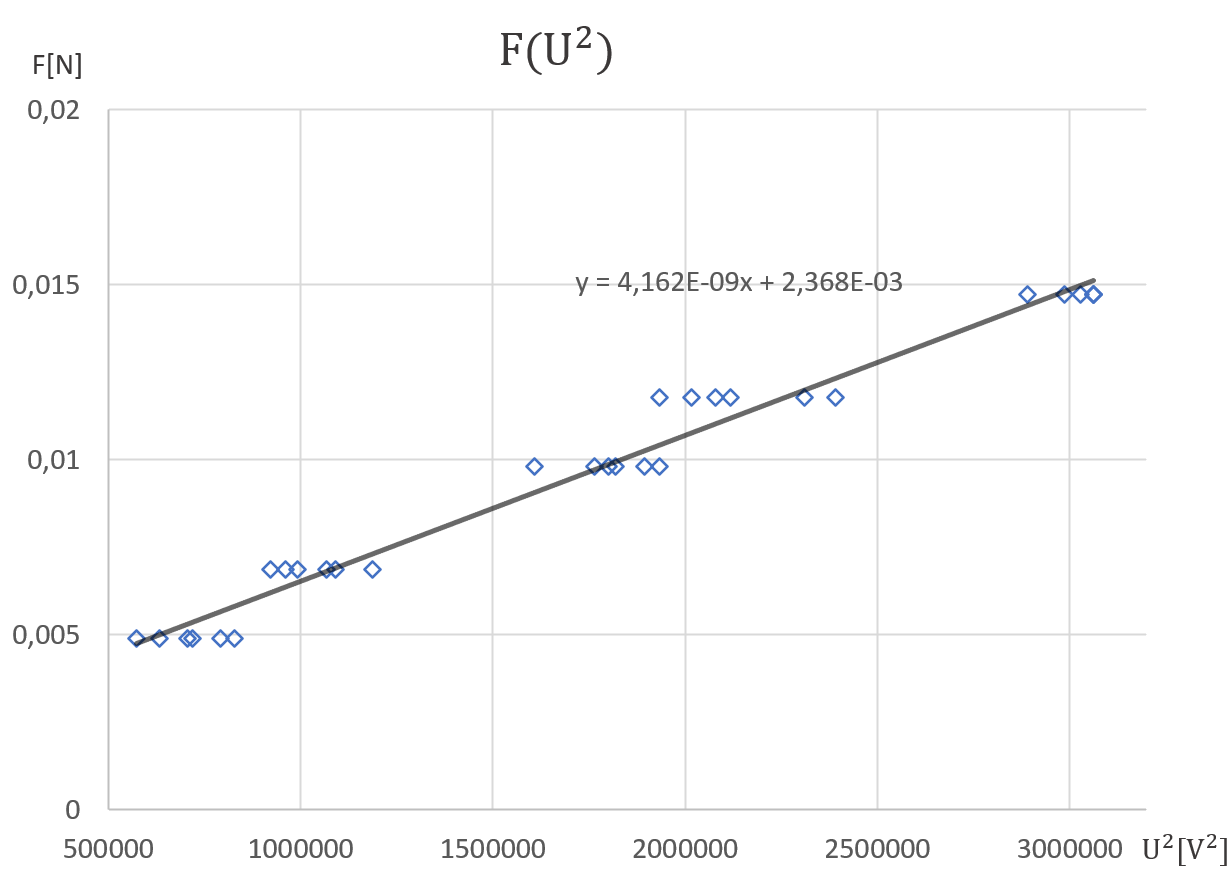
\includegraphics[width=\textwidth]{energija in frekvenca graf.png}

\end{figure}

\noindent Iz grafa dobimo koeficient $k = 4,16 \cdot 10^{-9} \frac{N}{V^2}$. Po enačbi $\varepsilon_0 = k\frac{2d^{2}}{S}$  dobimo

 \[\varepsilon_{0, merjen} = 7,6 \cdot10^{-12} \frac{F}{m} \pm 0.5 \cdot 10^{-12} \frac{F}{m}\]

\noindent Dejanska vrednost konstante je 8.85 $\cdot 10^{-12}$ $\frac{F}{m}.$ 

\chapter*{Dodatek}
Z uporabo dobro poznanega $\varepsilon_0$ lahko po enačbi

\[d=\sqrt{\varepsilon_0\frac{S}{2k}}\]

\noindent izračunamo natančnejši d kot

\[ d_{izracunan} = 0,55cm \pm 0,06cm\]
 

\end{document}